\documentclass[12pt,a4paper]{article}
\usepackage[utf8]{inputenc}
\usepackage[T1]{fontenc}
\usepackage[brazil]{babel}
\usepackage{lmodern}
\usepackage[margin=1.7cm,top=1.4cm,bottom=1.5cm]{geometry}
\usepackage{graphicx}
\usepackage{booktabs}
\usepackage{tabularx}
\usepackage{makecell}
\usepackage{amsmath}
\usepackage{caption}
\usepackage{enumitem}
\usepackage{microtype}
\usepackage{titlesec}
\titleformat*{\section}{\normalsize\bfseries}
\titlespacing*{\section}{0pt}{7pt}{2pt}
\setlist{nosep,leftmargin=*}
\captionsetup{font=small,labelfont=bf,skip=3pt}
\setlength{\parskip}{3pt}
\setlength{\parindent}{0pt}
\pagestyle{plain}

\begin{document}

{\large\textbf{Uma primeira investigação com o FD001: remoção por idade \textit{vs.} regra baseada em T50}}\\[2pt]
\small TE-292 --- Ciência de Dados em Operação e Manutenção de Aeronaves (ITA) $\cdot$ Prof.\ Antonio Celio Pereira de Mesquita $\cdot$ Aula 7 $\cdot$ \textbf{Aluno:} João Paulo Gomes de Oliveira\\
\small Código reprodutível: \texttt{tarefa\_fd001.ipynb} (mesma pasta).
\normalsize

\section*{1. Pergunta, contexto e protocolo}
Uma regra baseada em sensores aproveita melhor a vida do motor do que uma remoção por idade? O sensor usado é o \textbf{T50}
(sensor 4, coluna 9), a temperatura na saída da turbina de baixa pressão, em °R (Saxena et al., 2008, tab.~2). No FD001, o desgaste
do compressor de alta pressão faz o motor trabalhar mais quente, e o T50 sobe lentamente ao longo da vida. A decisão é lida pela
\textbf{curva P--F} da aula: o aviso marca o ponto P detectado, e a remoção chega a tempo se o intervalo $T-\text{aviso}$ for de pelo
menos $L=20$ ciclos. O custo por ciclo $\sum C/\sum U$ estima, pelo teorema da renovação com recompensa, o custo de longo prazo por
ciclo voado (Mesquita, aula~7). Os parâmetros são $c_p=1$ e $c_f=50$. Uma remoção até $T$ (inclusive) é planejada, com $U$ igual
ao ciclo da remoção e $C=1$. Remoção após $T$, ou ausência de aviso, conta como planejamento perdido, com $U=T$ e $C=50$.
\textbf{Protocolo:} usei apenas \texttt{train\_FD001.txt}. Os 100 motores foram sorteados com semente 42 em \textbf{70 de
desenvolvimento} e \textbf{30 reservados}, com todos os ciclos de cada motor no mesmo grupo. Os parâmetros foram escolhidos só nos
70, e as regras fixadas foram aplicadas \textbf{uma única vez} aos 30. O ciclo $T$ serve apenas para conferir o desfecho.

\section*{2. Regras}
\textbf{Idade.} $a$ = menor vida nos 70 motores $=$ \textbf{128 ciclos}: aviso em 108 e remoção em 128 para todos. Uma varredura
de $a$ nos 70 motores mostra que 128 é também a idade de \emph{menor custo por ciclo}, como na aula. A referência, portanto, é a
\textbf{melhor} política por idade, e a comparação é justa.

\textbf{Sensor.} É a regra de detecção do ponto P de Bassani (2026, slide~16), usando só o limite superior. A linha de base é a
média de T50 nos ciclos 1--15. A partir do ciclo 16, a média móvel usa as 15 leituras mais recentes, incluindo a atual. O aviso é
único e sai quando a média móvel supera a linha de base $\times(1+p)$; a remoção vem 20 ciclos depois. Nos 70 motores
(Tab.~\ref{tab:dev}), \textbf{$p=0{,}35\%$} teve o menor custo. O intervalo P--F explica o dilema. Com 0,50\%, o P--F mediano é de
57 ciclos e o mínimo de 19, abaixo de $L$; isso reproduz o padrão da aula (54 e 22 ciclos), e o único motor perdido custa 50. Com
0,20\%, o aviso sai cedo demais.

\begin{table}[h]
\centering\footnotesize
\caption{Seleção do percentual --- somente nos 70 motores de desenvolvimento.}\label{tab:dev}
\setlength{\tabcolsep}{5pt}
\begin{tabular}{lccccc}
\toprule
Regra & Perdidos/70 & Desperdício médio & P--F mediano & P--F mín. & Custo/ciclo\\
\midrule
Sensor, $p=0{,}20\%$ & 0 & 100,9 & 116 & 55 & 0,00953\\
\textbf{Sensor, $p=0{,}35\%$ (escolhido)} & \textbf{0} & \textbf{68,3} & \textbf{78} & \textbf{43} & \textbf{0,00727}\\
Sensor, $p=0{,}50\%$ & 1 & 43,6 & 57 & 19 & 0,01044\\
Idade, $a=128$ & 0 & 77,8 & --- & --- & 0,00781\\
\bottomrule
\end{tabular}
\end{table}

\section*{3. Resultado nos 30 motores reservados}
\begin{table}[h]
\centering\small
\caption{Comparação final (regras fixadas antes da avaliação, aplicadas uma única vez).}\label{tab:aval}
\begin{tabularx}{\linewidth}{Xccc}
\toprule
Regra & \makecell{Motores com plane-\\jamento perdido / 30} & \makecell{Vida desperdiçada média,\\só nas remoções planejadas} & Custo por ciclo\\
\midrule
Remoção por idade ($a=128$) & 0 / 30 & 79,5 ciclos & 0,00781\\
Regra baseada em sensores (T50, $+0{,}35\%$) & 0 / 30 & 71,7 ciclos & \textbf{0,00737}\\
\bottomrule
\end{tabularx}
\end{table}

O custo por ciclo caiu \textbf{5,7\%}, sem planejamento perdido em nenhuma das regras. O sensor aproveitou, em média, 135,8 ciclos
por motor, contra 128 da idade. A dispersão da folga $T-$remoção caiu de 43,2 para 35,3 ciclos, e a menor folga foi de 28 ciclos.
A Figura~\ref{fig:motor} mostra o motor 9, escolhido por um critério objetivo: é o motor reservado com vida mais próxima da mediana.

\begin{figure}[h]
\centering
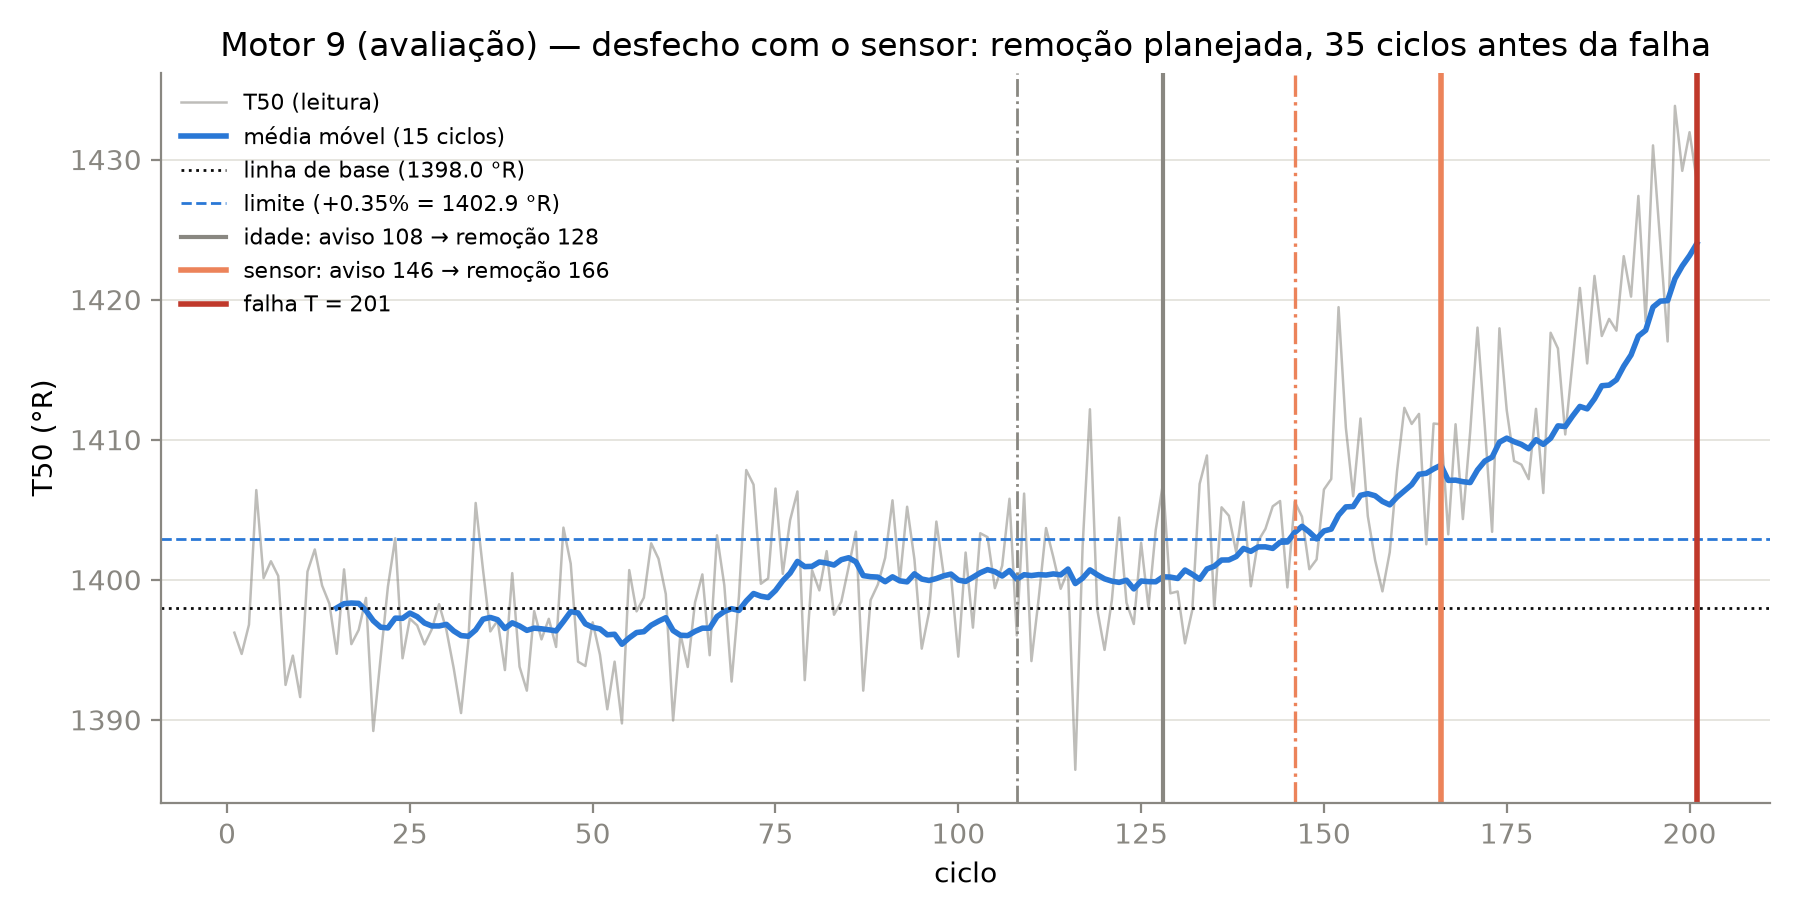
\includegraphics[width=0.68\linewidth]{figuras/motor_exemplo.png}
\caption{Motor 9 (avaliação): T50, média móvel, linha de base e limite de $+0{,}35\%$. As linhas tracejadas marcam os avisos e as
linhas cheias marcam as remoções (cinza: idade; laranja: sensor). A linha vermelha marca a falha. O sensor remove 35 ciclos antes da
falha; a idade, 73 ciclos antes.}\label{fig:motor}
\end{figure}

\section*{4. Conclusão e limitação}
\textbf{A regra com sensor melhorou a decisão, mas de forma modesta e ainda não conclusiva.} No bootstrap pareado dos 30 motores
(5000 reamostras), a razão entre os custos por ciclo (sensor $\div$ idade) é 0,94, com IC95\% de [0,88; 1,02]. O sensor é mais barato
em 94\% das reamostras, mas o intervalo inclui 1. O ganho vem de personalizar a remoção, enquanto a idade trata todos os motores como
o pior caso. Essa personalização é \textbf{parcial}: o ciclo de remoção tem correlação de apenas $r=0{,}58$ com a vida real, e o motor
7 (vida de 259 ciclos) sai no ciclo 100, porque o ruído leva a média móvel a cruzar um limite pequeno. \textbf{Limitação:} a escolha
de $p$ foi decidida por \emph{um único motor} no desenvolvimento, aquele que 0,50\% perdeu. Com $c_f=50$, uma remoção tardia inverte o
resultado, e com 30 motores a incerteza do custo é da mesma ordem que a diferença encontrada.

\section*{5. Próxima investigação}
\textbf{Ideias do artigo} (Saxena et al., 2008). A seção V.A (p.~5) explica que cada motor começa com desgaste inicial e variação de
fabricação diferentes; isso justifica a linha de base \emph{por motor}. A seção V.B (p.~5) descreve o ruído de mistura que mascara a
degradação; isso explica os avisos precoces. A seção VII (pp.~7--8) penaliza mais o erro tardio, a mesma assimetria de $c_f/c_p=50$.
Antes de formular a pergunta, comparei nos \emph{70 motores de desenvolvimento} as alternativas da aula (slide~32). Com o T50
isolado, o limiar estatístico $(\bar x-\mu)/(\sigma/\sqrt{15})>k$ não supera 0,35\%: o próprio $\sigma$ de 15 leituras é ruidoso.
Já a média dos desvios relativos de \textbf{T50 e Ps30} (pressão na saída do HPC) chegou a custo 0,0064, sem perdas e com $r=0{,}90$.
Esse valor, porém, é \emph{in-sample} e sujeito ao otimismo de seleção apontado na aula (slide~42).

\textbf{O que mudaria:} no próximo experimento, eu combinaria T50 e Ps30 nessa média de desvios relativos. O limite seria escolhido
por validação cruzada interna nos 70 motores, e a regra fixada seria aplicada uma única vez aos mesmos 30 motores reservados. A
mudança terá ajudado se, nesses 30 motores, a correlação entre o ciclo de remoção e $T$ superar 0,58, o custo por ciclo ficar
abaixo de 0,00737, com o IC95\% do bootstrap pareado contra a regra atual abaixo de 1, e o número de planejamentos perdidos não
aumentar.

\vspace{2pt}\footnotesize\textbf{Referências.} Saxena, A.; Goebel, K.; Simon, D.; Eklund, N. \emph{Damage Propagation Modeling for
Aircraft Engine Run-to-Failure Simulation}. PHM08, 2008. --- Mesquita, A.\,C.\,P. \emph{Quando remover o motor? O conjunto C-MAPSS e o
planejamento de manutenção com antecedência logística}. TE-292, aula 7, ITA, 2026. --- Bassani, A.\,S. Defesa de mestrado, ITA,
5/10/2026 (detecção do ponto P em T50, slide 16).

\end{document}
